\section{工作原理}
BLXLRSMB是一个3D显示设备。
通过电机驱动PCB板高速旋转,在特定角度点亮板上的特定彩灯,实现三维显示的效果。
\begin{center}
  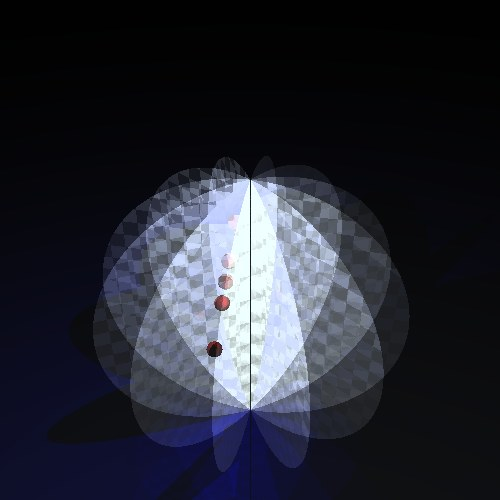
\includegraphics[scale=0.4]{../img/concept.jpg}
\end{center}

在旋转的PCB板上设置了一个红外接收器,接收下方固定位置红外发射器的信号,通过
两次信号的时间差计算当前旋转的角度。

对每一个特定角度,从UFM中读取预先由软件计算出的各帧图形数据,显示在灯阵上,形成三维效果。

